\documentclass{subfiles}
\begin{document}
\section{General study of basis sets and numerical methods}\label{sec:general_study_results}
\textcolor{red}{TODO: Clean up this section. Are we happy with title?}
\subsection{Sinc-DVR basis validation}
\subsubsection*{Energy eigenstates}
A natural validation of the Sinc-DVR basis is to check that the Sinc-DVR basis functions closely match the exact energy eigenstates of the system. We require that the functions that the Sinc-DVR basis is constructed to have a high degree of overlap with the exact energy eigenstates of the system. Otherwise, we risk losing important information about dynamics of the system, dynamics that may have a significant impact on the quantum control protocols we wish to implement.\\ 

We begin by computing the overlap matrix $S$ between the Sinc-DVR basis functions and the exact energy eigenstates of the Morse potential. Recall, the overlap matrix is defined as:
\begin{align*}
    S_{ij} = \int \psi_i(x) \psi_j(x) dx,
\end{align*}
where $\psi_i(x)$ and $\psi_j(x)$ are the Sinc-DVR basis and exact energy eigenstates, respectively.\textcolor{red}{TODO: Should ref this better to prior sections. SHould we add the assessment section that could bind this?} 

The overlap matrix $S$ is then a measure of how well the Sinc-DVR basis functions represent the exact energy eigenstates of the system. The results are shown in figure \ref{fig:dvr_validation_overlap}, where we see that the overlap between the Sinc-DVR basis functions and the exact energy eigenstates is quite high, especially for the lowest lying states. We see that the overlap matrix is close to the identity matrix, indicating a near perfect overlap between the two basis sets.
\begin{figure}[h!]
    \centering
    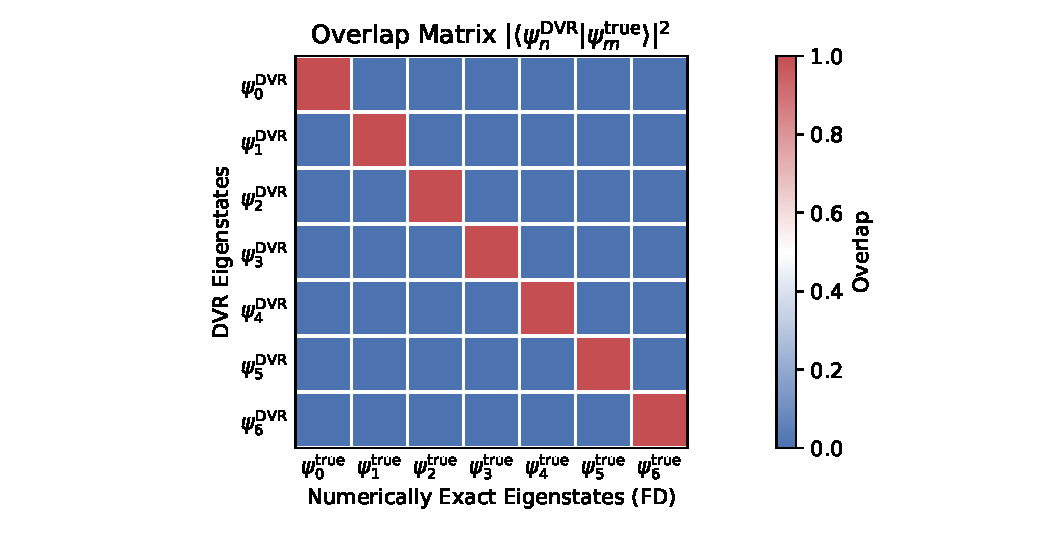
\includegraphics[width=\textwidth]{figs/dvr_validation_overlap.pdf}
    \caption{Overlap between the Sinc-DVR basis functions and the exact energy eigenstates of the Morse potential. The parameters used for the Morse potential are $D = 10.0$, $a = 1.0$, and $x_0 = 0.0$. The grid spacing is $\Delta x = 0.025$, and the number of grid points is $N = 200$.}
    \label{fig:dvr_validation_overlap}
\end{figure}
\\
Qualitatively, we see near perfect overlap between the Sinc-DVR basis functions and the exact energy eigenstates of the system. We note that the exact energy eigenstates are computed using finite-differences to approximate the spatial derivate in the Schrödinger equation \eqref{eq:TISE}, and thus, they are not exact outside the numerical tolerance of the finite-difference method. However, with our choice of grid spacing and number of grid points, we assume a high degree of accuracy in the finite-difference method, and thus, we can safely assume that the Sinc-DVR basis functions closely match the exact energy eigenstates of the system. Quantitatively, the diagonal elements of the overlap matrix exceed $0.9999$ for the lowest lying states, indicating a fidelity of $99.99\%$ or higher, which is more than sufficient for our study.  Even with our semi-course grid spacing of $\Delta x = 0.025$ a.u., we maintain the same level of fidelity for the higher order states, with the diagonal elements of the overlap matrix exceeding $0.9995$ for the first 20 energy eigenstates (we restrict Figure \ref{fig:dvr_validation_overlap} to the first 7). Such strong agreement means we can trust the Sinc-DVR basis to accurately represent the dynamics of in our quantum control protocols. 

\subsubsection*{Energy spectrum}
Next, we compute the energy spectrum of the Morse potential using the Sinc-DVR basis and compare it to the exact energy eigenvalues, found using finite-differences to approximate the spatial derivate in the Schrödinger equation \eqref{eq:TISE}\textcolor{red}{TODO: Add a minor section on finite-differences?}. We follow the procedure outlined in section \ref{sec:sinc_dvr_validation}, and the resulting energies are shown in figure \ref{fig:dvr_validation}. The energy spectrum is shown in atomic units, and we see that the energy levels of the Sinc-DVR basis closely align with the exact energies of the system, especially for the lowest lying states - of which we are mostly interested in. 
\begin{figure}[h!]
    \centering
    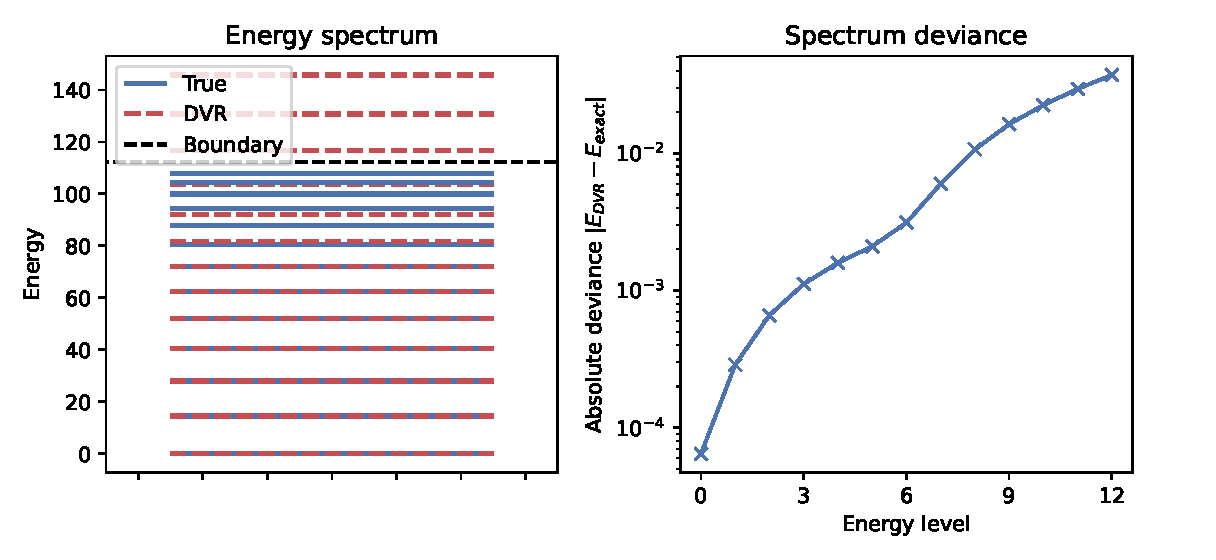
\includegraphics[width=\textwidth]{figs/dvr_validation.pdf}
    \caption{Comparison of the energy spectrum of the Morse potential using the Sinc-DVR basis and the exact energy eigenstates. The parameters used for the Morse potential are $D = 10.0$, $a = 1.0$, and $x_0 = 0.0$. The grid spacing is $\Delta x = 0.025$, and the number of grid points is $N = 200$. The energy spectrum is shown in atomic units. The absolute deviances is plotted logarithmically.}
    \label{fig:dvr_validation}
\end{figure}

The DVR reproduces the ground-state energy to within $10^{-5}$ a.u., and the first two excited states to within $10^{-4}$ a.u. As seen in Figure \ref{fig:dvr_validation}, the absolute deviances of the energy eigenvalues are plotted logarithmically, and the first 6 eigenlevels have a relative error below $10^{-2}$. The increasing error for the higher order states is expected, and is a result of the spectral convergence of the Sinc-DVR basis. As we are mostly interested in the lowest lying states, we do not mind the increasing error for the higher order states, as they are not relevant for our quantum control protocols. \textcolor{red}{TODO: Check over the arguments in this paragraph. Should we discuss moe on the spectral convergence of the Sinc-DVR basis? Probably could use a detailed discussion in the theory section instead.}
\subsubsection{Implications and convergence}
Taken together, the near-perfect overlaps and sub-Hartree energy errors demonstrate that the Sinc-DVR basis intoduce negligible residual errors in the representation of the energy eigenstates and the energy spectrum of interest in the Morse potential. If we desire, we may further reduce the error by inceasing the number of grid points $N$ (or decreasing the grid spacing $\Delta x$). We therefore proceed with confidence that the Sinc-DVR basis is a suitable choice for our quantum control protocols, as it accurately captures the essential features of the system.

\subsection{Numerical methods: Landau-Zener model}
To systematically validate our implementation of the aforementiond numerical methods (Section \ref{sec:time_evolve_methods}), we require a simple yet representative quantum system that exhibits non-trivial dynamics but still has closed form solutions for comparison. For this purpose, we will once again turn to the simple Landau-Zener model \eqref{eq:landau_zener}, introduced in the section on avoided crossings \ref{sec:avoided_crossings}. This simple two-level system is governed by a time-dependent Hamiltonian. It captures the essential features of quantum dynamics, making it an ideal testbed for our numerical methods in preparation for the more complex double-well Morse potential system we shall study.
Recall, the Hamiltonian for the Landau-Zener model is given by:
\begin{align*}
    H(t) = \begin{pmatrix}
        vt & V \\
        V & -vt
\end{pmatrix},
\end{align*}
where $v$ is the sweeping velocity, $V$ is the coupling strength, and $t$ is the time. At $t=0$, the uncoupled system would have a degeneracy, but the coupling $V$ opens a gap (lifts the degeneracy), resulting in an avoided crossing as we saw in section \ref{sec:avoided_crossings}. Thus, this minimal system captures one of the simplest non-trivial dynamics of a quantum system which also leads to a well known analytical solution for the transition probability \eqref{eq:landau_zener_trans_prob}. 

This system is particularly useful for validating our numerical methods, and serves as a suitable testbed for benchmarking due to several reasons, of which some are listed below:
\begin{itemize}
    \item \textbf{Low dimensionality:} The Landau-Zener model is a two-level system, making it computationally efficient to simulate and analyze. This allows us to focus on the numerical methods without being overwhelmed by the computational complexity of the system.
    \item \textbf{Non-trivial dynamics:} The system exhibits interesting dynamics, such as transitions betweeen states, which require the numerical implementations to accurately capture the time evolution of the wavefunction. This provides a meaningful test for the accuracy and stability of the numerical methods.
    \item \textbf{Analytical reference:} The Landau-Zener model has well-known analytical solutions for the transition probabilities and wavefunction dynamics, allowing us to directly compare the results of our numerical methods against these exact solutions. This serves as a benchmark for assessing the performance of the numerical methods.
\end{itemize}
\subsubsection*{Benchmark procedure}
We initialize the system in the lowest lying diabatic state $\ket{\Psi(0)} = \begin{pmatrix} 1 \\ 0 \end{pmatrix}$, which corresponds to the ground state of the uncoupled system, from an initial time $t_0<0$ to a final time $t_f>0$. We will then compare:
\begin{itemize}
    \item Global error vs. simulation time $T$: How the methods converge towards the closed form solution.
    \item Runtime efficiency: How fast each method can compute the transition probability.
    \item Stability during evolution: How well each method handles long time simulations. 
\end{itemize}
\\ 
We numerically propagate an initial wavefunction prepared in the ground state of the uncoupled system (the \emph{diabatic basis}), and compute the final transition probability $P_{12}$, given analytically by \eqref{eq:landau_zener_trans_prob}. In other words, after the sweep we compute 
\begin{align*}
    P_{1\to2} = |\braket{\Psi_2|\Psi(t_f)}|^2,
\end{align*}
the probability of finding the system in the excited diabatic state $\ket{\Psi_2}$ at time $t_f$, given that it was initially prepared in the ground diabatic state $\ket{\Psi_1}$. This process is repeated for various numerical methods using a fixed time step $\Delta t$, while varying the length of simulation $2T$. The Landau-Zener transition probability is derived in the infinite time-limit, i.e $t\rightarrow \pm \infty$, so this analysis illustrate how each numerical method converges to the analytical solution as the simulation time increases.
\begin{figure}[h!]
\centering
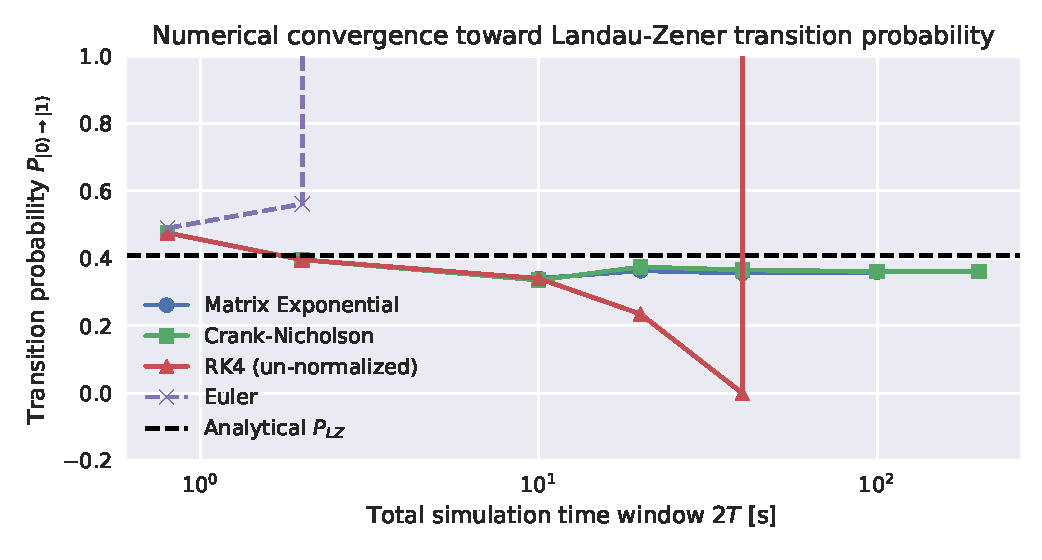
\includegraphics[width=1.0\textwidth]{figs/landau_zener_convergence_benchmark.pdf}
\caption{Final transition probability computed using various numerical methods for increasing total simulation time $
2T$. All methods converge toward the analytical Landau-Zener probability (dashed line), with RK4 showing good accuracy until instability sets in at longer times due to lack of normalization. Euler becomes unstable very early. The x-axis is in logarithmic scale.}
\end{figure}

As we can see in figure \eqref{fig:landau_zener_convergence_benchmark}, the methods converge towards the analytical solution within certain timeframes, with varying degrees of stability. The two Taylor-expansion methods (Euler and RK4) show good agreement for shorter timeframes but quickly become unstable, with Euler diverging rapidly, which is expected since we've seen this behaviour already in figure \eqref{fig:landau_zener}. The more robust RK4 method remain stable and follow closely with the more sophisticated methods, before the accumulated error in the norm blows it up. Both of these methods can be improved upon by introducing norm corrections, at a computational cost (albeit minimal). The Crank-Nicolson method, on the other hand, remains stable and accurate for longer simulation times, as it preserves unitarity by construction. 
\\ 

To assess the computational speed of the numerical methods, a full Landau-Zener simulation was measured using the \texttt{time.perf\_counter()} function in Python, which provides a high-resolution timer suitable for short time measurements.This measurement also includes system overhead, yielding realistic performance metrics to evaluate each method. 
The benchmark was performed for the two-level system with sweeping parameter $v=7.0$, coupling strength $V=1.0$, and a time integration interval of $t \in [-5, 5]$ with $100{,}000$ time steps, i.e a time-step of $\Delta t = 10^{-4}$s. The results are presented in the following table \eqref{tab:landau_zener_runtime}, which summarizes the runtime of each method, along with remarks on their performance characteristics.

\begin{table}[h!]
\centering
\caption{Runtime comparison of time propagation methods for the Landau-Zener model ($v = 7.0$, $\Delta = 1.0$, $t \in [-5, 5]$, 100,000 steps). Timing measured using \texttt{time.perf\_counter()}.}
\begin{tabular}{l c l}
\toprule
\textbf{Method} & \textbf{Time (ms)} & \textbf{Remarks} \\
\midrule
Matrix Exponential & 5942.1 & Most accurate, but very slow \\
Euler              & 828.6  & Fastest, but unstable \\
RK4                & 2621.0 & Balanced performance \\
Crank--Nicholson   & 1953.6 & Stable and efficient \\
\bottomrule
\end{tabular}\label{tab:landau_zener_runtime}
\end{table}
The table \eqref{tab:landau_zener_runtime} shows that the matrix exponential method is the slowest, but also it is exact, while the Euler method is the fastest but unstable and inaccurate for longer simulations. The RK4 method is a good compromise between speed and accuracy, while the Crank-Nicolson method is stable and efficient, but slower than RK4. 

In conclusion, the convergence converges together with the runtime analysis shows that the Crank-Nicolson method is the most suitable for long time simulations, as it preserves unitarity and stability, for cases where direct matrix exponentiation is not feasible. We have confirmd that the explicit Taylor-expansion methods (Euler and RK4) can work over shorter intervals, they require norm corrections, and small time steps to remain reliable. Direct matrix exponentiation is unbeatable with regards to accuracy, but scales exponentially in computational cost. Crank-Nicolson hits a sweet spot: It is unconditionally stable, preserves unitarity, and is computationally efficient for long time simulations. 

Because our goal is to simulate two interacting particles trapped in a double-well potential, in a Hartree-reduced basis, we choose to employ direct matrix exponentiation whenever possible, and to default Crank-Nicolson for extended time-simulations. While one could explore more advanced methods, we firmly believe that the Crank-Nicolson method is sufficient for our purposes, as it provides a good balance between accuracy, efficiency and simplicity.
\end{document}